\documentclass{astroedu-lab}

\begin{document}

\pagestyle{plain}

\begin{problem}{\huge Лабораторная работа 4.7.3\\\\Поляризация\\\\Выполнил Жданов Елисей Б01-205}

\section{Цель работы:}

Ознакомление с методами получения и анализа поляризованного света.

\section{Оборудование:}

Оптическая скамья с осветителем; зелёный светофильтр; два поляроида; чёрное зеркало; полированная эбонитовая пластинка; стопа стеклянных пластинок; слюдяные пластинки разной толщины; пластинки в 1/4 и 1/2 длины волны; пластинка в одну длину волны для зелёного света (пластинка чувствительного оттенка).

\section{Теоретическая справка}

\subsection{Определение направления разрешённой плоскости колебаний поляроида}
	
	Определить направление разрешённых колебаний поляроида проще всего с помощью чёрного зеркала.
	
При падении света на отражающую поверхность под углом Брюстера, свет в отражённом луче почти полностью поляризован, а вектор E
параллелен отражающей поверхности ("<правило иголки">). Луч света,
прошедший поляроид и отразившийся от чёрного зеркала, имеет минимальную интенсивность при выполнении двух условий: во-первых, свет
падает на отражающую поверхность под углом Брюстера и, во-вторых,
в падающем пучке вектор E лежит в плоскости падения.

Вращая поляроид вокруг направления луча и чёрное зеркало вокруг
оси, перпендикулярной лучу, методом последовательных приближений
можно добиться минимальной яркости луча, отражённого от зеркала,
и таким образом определить разрешённое направление поляроида.

Измеряя угол поворота зеркала (угол Брюстера), нетрудно определить коэффициент преломления материала, из которого изготовлено
зеркало. Описанный метод часто используется для измерения коэффициента преломления непрозрачных диэлектриков.

\subsection{Получение эллиптически поляризованного света}
\begin{wrapfigure}{r}{0.35\linewidth} 
	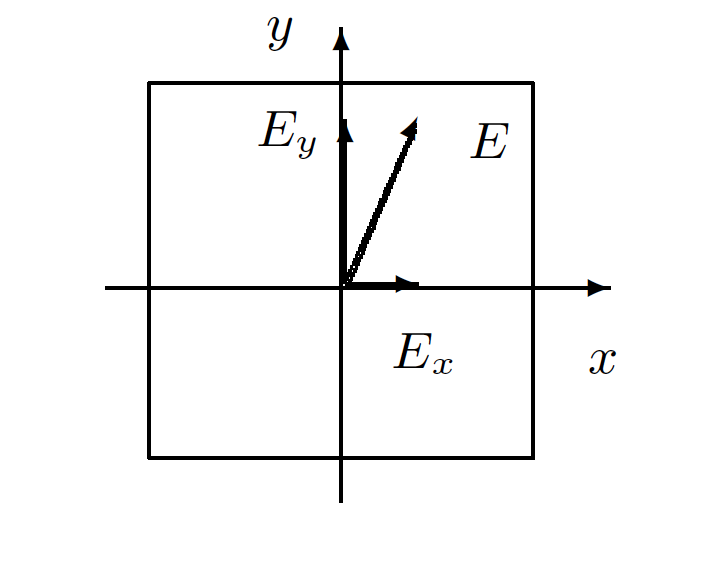
\includegraphics[width=\linewidth]{1}
	\caption{Разложение линейно поляризованного света по главным направлениям двоякопреломляющей пластинки}
	\label{ris 1}
\end{wrapfigure}

Эллиптически поляризованный свет можно получить из линейно поляризованного с
помощью двоякопреломляющих кристаллических пластинок.

Двоякопреломляющая пластинка имеет два взаимно перпендикулярных главных направления, совпадающих с осями эллипсоида диэлектрической проницаемости. Волны, поляризованные вдоль главных направлений, распространяются в пластинке с разными скоростями, не изменяя характера своей поляризации. Эти волны называются главными. Мы будем обозначать показатели преломления для главных волн через $ n_x $ и $ n_y $, где $ x $ и $ y $ --- главные направления кристаллической пластинки (рис. 1).

Пусть на пластинку падает линейно поляризованная волна, электрический вектор которой ориентирован под некоторым углом $ \alpha $ к оси
$ x $. Разложим вектор $ \mathbf{E} $ на составляющие $ E_x $ и $ E_y $. На входе пластинки $ E_x $ и $ E_y $ находятся в фазе. На выходе из-за разности скоростей между ними появляется разность хода $ d(n_x - n_y) $, при этом сдвиг фаз определяется соотношением

\begin{equation}\label{}
\Delta \phi =  \dfrac{2\pi}{m} = k d(n_x - n_y)
\end{equation}
Как уже отмечалось, при сложении двух взаимно перпендикулярных колебаний, обладающих некоторым сдвигом фаз, образуется колебание, поляризованное по эллипсу.

\newpage

\begin{wrapfigure}{l}{0.35\linewidth}
	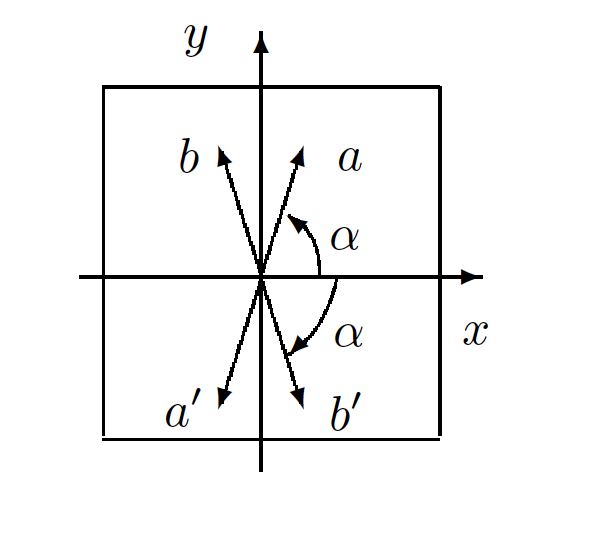
\includegraphics[width=\linewidth]{2}
	\caption{Поворот направления колебаний с помощью пластинки в $ \lambda / 2 $}
	\label{ris 2}
\end{wrapfigure}


Рассмотрим практически важные частные случаи.

 		
1) Пластинка даёт сдвиг фаз $ 2\pi $ (пластинка в длину волны $ \lambda $). В результате сложения волн на выходе пластинки образует-
ся линейно поляризованная волна с тем же направлением колебаний, что и в падающей волне.

2) Пластинка даёт сдвиг фаз $ \pi $ (пластинка в полдлины волны $ \lambda / 2 $). На выходе пластинки снова образуется линейно поляризованная волна. Направление $ bb' $ колебаний этой волны повёрнуто относительно направления $ aa' $ колебаний падающей волны (рис. 2). Как нетрудно сообразить, направление $ bb' $ является зеркальным отображением направления $ aa' $ относительно одного из главных направлений пластинки. Такую пластинку используют для поворота направления колебаний линейно поляризованного света.

3) Пластинка создаёт между колебаниями сдвиг фаз $ \pi/2 $ (пластинка
в четверть длины волны). При сложении двух взаимно перпендикулярных колебаний, имеющих разность фаз $ \pi/2 $, образуется эллипс, главные оси которого совпадают с координатными осями $ x $ и $ y $. При равенстве амплитуд возникает круговая поляризация.

Следует отметить, что, говоря о пластинках $ \lambda , \lambda/2, \lambda/4  $ и т. д., всегда подразумевают какую-либо вполне определённую монохроматическую
компоненту (например, пластинка $ \lambda/2 $ для зелёного света). Если на двоякопреломляющую пластинку падает не монохроматический свет, то на
выходе из неё для разных спектральных компонент эллипсы поляризации будут различными.

\subsection{Анализ эллиптически поляризованного света}

Анализ эллиптически поляризованного света сводится к нахождению главных осей
эллипса поляризации и к определению направления вращения электрического вектора.

Главные оси эллипса поляризации определяются с помощью анализатора по максимуму и минимуму интенсивности проходящего света.
Направление вращения электрического вектора может быть найдено
с помощью пластинки в четверть длины волны, для которой известно,
какая из главных волн, $ E_x $ или $ E_y $, имеет б\'{o}льшую скорость распространения (и соответственно меньшее значение показателя преломления).

Выберем для определённости координатные оси x и y на пластинке
так, чтобы $ nx < ny $. В этом случае главная волна $ E_x $ имеет большую
скорость распространения. Поместим такую пластинку на пути эллиптически поляризованного света и совместим главные направления пластинки $ \lambda/4 $ с главными осями эллипса поляризации. На выходе из этой
пластинки сдвиг фаз между $ E_x $ и $ E_y $ вместо $ \pi/2 $ станет равным ну-
лю или $ \pi $. Свет окажется линейно поляризованным. Из двух возможных значений сдвига фаз, 0 или $ \pi $, реализуется одно: то, которое соответствует имеющемуся в волне направлению вращения электрического вектора.

Рассмотрим, например, случай, когда электрический вектор в эллиптически поляризованной волне вращается против часовой стрелки,
если смотреть навстречу лучу. В этом случае, очевидно, в волне, падающей на пластинку в $ \lambda/4 $, колебание $ E_y $ отстаёт по фазе на $ \pi/2 $ от
колебания $ E_x $. При прохождении через пластинку разность фаз увеличивается до $ \pi $. Таким образом на выходе из пластинки возникают линейно поляризованные волны со сдвигом фаз $ \pi $. Сложение этих волн
даёт плоскополяризованную волну, электрический вектор которой рас-
полагается во втором и четвёртом квадрантах координатной системы
$ x, y $.

Рассуждая аналогичным образом, найдём, что при вращении электрического вектора по часовой стрелке направление колебаний в линейно поляризованной волне, выходящей из пластинки, располагается в первом и третьем квадрантах. Определяя направление колебаний на выходе из пластинки с помощью поляроида, можно, таким образом, определить характер эллиптической поляризации (вращение против или по часовой стрелке).

\subsection{Пластинка чувствительного оттенка}

\begin{wrapfigure}{l}{0.35\linewidth}
	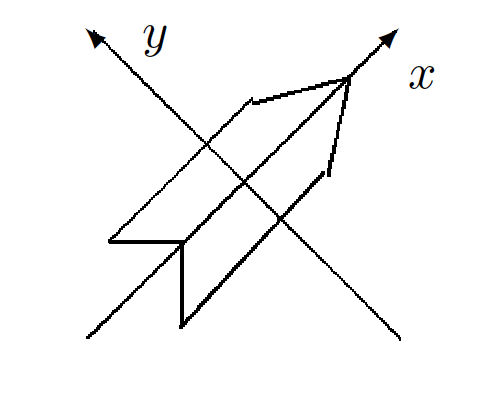
\includegraphics[width=\linewidth]{3}
	\caption{Пластинка
чувствительного
оттенка}
	\label{ris 3}
\end{wrapfigure}

Выше предполагалось известным, какому из двух главных направлений пластинки в четверть длины волны соответствует большая скорость распространения света.
Установить это можно различными способами, например с помощью
пластинки чувствительного оттенка (так называют пластинку в $ \lambda $
для зелёной спектральной компоненты, $ \lambda = 560 $ нм).

Пластинка имеет форму стрелы (рис. 3), вдоль оси которой расположено главное направление, соответствующее большей скорости распространения.

Если пластинка чувствительного оттенка помещена между скрещенными поляроидами и главные направления пластинки не параллельны
направлениям разрешённых колебаний поляроидов, то при освещении
белым светом пластинка кажется окрашенной в лилово-красный цвет.
Это объясняется тем, что зелёная компонента линейно поляризованного света при прохождении пластинки не меняет поляризации и задерживается вторым поляроидом. Для красной и фиолетовой компонент
пластинка создаёт сдвиг фаз, несколько отличный от $ 2\pi $. На выходе
из пластинки красная и фиолетовая компоненты оказываются поэтому
эллиптически поляризованными и частично проходят через второй поляроид. Таким образом, в известном смысле наблюдаемый в указанном
опыте цвет пластинки дополнителен к зелёному.

Если между скрещенными поляроидами поместить пластинку чувствительного оттенка
($ \lambda $) и пластинку в $ \lambda/4 $ так, чтобы их главные
направления совпадали, цвет пластинки изменится. Если у пластинки чувствительного оттенка и пластинки в $ \lambda/4  $совпадут главные направления, соответствующие большей скорости распространения, то разность хода между $ E_x $ и $ E_y $ для зелёного света составит уже $ 5\lambda/4 $. Это соответствует разности хода в $ \lambda $ для света с большей длиной волны, т. е. для "<более красного"> света. При освещении
этих пластинок (напомним, что они расположены между скрещенными поляроидами) белым светом теперь погасится не зелёная, а красная
часть спектра, и проходящий свет будет казаться зеленовато-голубым.
Если же главные направления, соответствующие большей скорости распространения, у пластинки чувствительного оттенка и у пластинки
в $ \lambda/4 $ окажутся перпендикулярными, то проходящий свет приобретёт
оранжево-желтую окраску (погасится фиолетово-голубая часть спектра).

Изменение цвета позволяет, таким образом, определить, какое из
главных направлений пластинки в $ \lambda/4 $ соответствует большей скорости распространения.

\subsection{Интерференция поляризованных лучей}

\begin{wrapfigure}{r}{0.35\linewidth}
	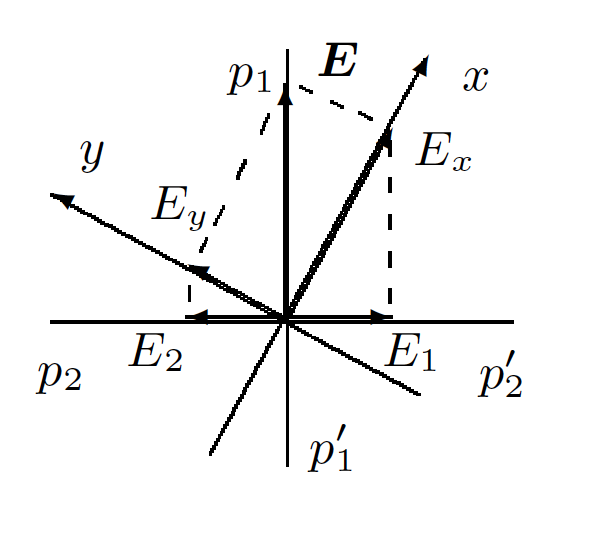
\includegraphics[width=\linewidth]{4}
	\caption{К объяснению интерференции
поляризованных лучей}
	\label{ris 4}
\end{wrapfigure}


Тонкие двоякопреломляющие пластинки, помещённые между поляроидами, кажутся окрашенными. Эта окраска может быть истолкована как результат интерференции поляризованных лучей. На рис. 4 представлена схема для
случая скрещенных поляроидов.

Здесь $ p1p'1 $ --- разрешённое направление колебаний поляризатора
(первого поляроида); $ x, y $ --- координатная система, связанная с главны-
ми направлениями двоякопреломляющей пластинки; $ p2p'2 $ --- разрешённое направление колебаний анализатора (второго поляроида). Волны
$ E_x  $ и $ E_y $ на выходе из пластинки когерентны, но не могут интерферировать, так как $ E_x \perp  E_y $. Волны $ E_1 $ и $ E_2 $ на выходе второго поляроида
также являются когерентными и к тому же поляризованы в одной плоскости. Эти волны интерферируют между собой. Результат интерференции определяется зависящим от длины волны сдвигом фаз между $ E_1 $
и $ E_2 $. В результате интерференции поляризованных лучей пластинка, освещаемая белым светом, кажется окрашенной.

Если поворачивать двоякопреломляющую пластинку, расположенную между
скрещенными поляроидами, то соотношение амплитуд волн $ E_1 $ и $ E_2 $ и разность фаз между ними не изменяются. Это означает, что цвет пластинки при её поворотах не меняется, а меняется только интенсивность света. За один оборот пластинки интенсивность четыре раза обращается в нуль --- это происходит при совпадении главных направлений
$ x $ и $ y $ с разрешёнными направлениями колебаний поляроидов.

Если же двоякопреломляющую пластинку оставить неподвижной, а
второй поляроид повернуть так, чтобы разрешённые направления $ p1p'1 $
и $ p2p'2 $ совпали, то волны $ E_1 $ и $ E_2 $ приобретают дополнительный фазовый сдвиг на $ \pi $ для всех спектральных компонент; при этом их амплитуды изменятся так, что цвет пластинки изменится на дополнительный. 

\section{Измерения, Обработка}

\subsection{Определение разрешённых направлений поляроидов}

Разместим на оптической скамье осветитель
S, поляроид P1 и чёрное зеркало.

Поворачивая поляроид вокруг направления луча, добьёмся наименьшей яркости отражённого пятна. Оставим поляроид в этом положении и вращением зеркала вокруг вертикальной оси снова добьёмся минимальной интенсивности отражённого луча

Для первого поляроида разрешённое направление горизонтальное, на лимбе

$\varphi_1 = 176^{\circ}$

Вместо чёрного зеркала поставим второй поляроид. Скрестив их, определим горизонтальное разрешённое направление второго поляроида, на лимбе

$\varphi_2 = 305^{\circ}$

\subsection{Определение угла Брюстера для эбонита}

Поставим на скамью вместо чёрного зеркала эбонитовую пластину с круговой шкалой и проведем подобные эксперименты по нахождению угла Брюстера.

Угол поворота эбонита, при котором интенсивность
отражённого луча минимальна: его абсолютное значение равно

$\varphi_\text{Б} = 55 \pm 1^{\circ}$ (погрешность цены деления)

Повторим измерения, добавив светофильтр Ф, и сравним результаты - они получились одинаковыми

По углу Брюстера рассчитаем показатель преломления эбонита и сравним с табличным.

\begin{center}
    $n = \tg \varphi = \tg 55^{\circ} = 1.43 \pm 0.05$
\end{center}

Табличное значение показателя преломления эбонита $n = 1.6$

По всей видимости, используется другой сорт материала, либо это вообще не эбонит.

\subsection{Исследование стопы}

Поставим стопу стеклянных пластинок вместо эбонитового зеркала под углом Брюстера.

Наблюдая прошедший через стопу стеклянных пластинок луч света, убедимся в том что плоскости поляризации у отраженного и преломленного лучей взаимно перпендикулярны (в прошедшем свете есть небольшая компонента вертикальной поляризации; это обусловлено тем, что небольшая часть вертикально поляризованного излучения все-же проходит через стопу, в отличие от горизонтальной, которая проходит через стопу практически вся).

\subsection{Определение главных плоскостей двоякопреломляющих пластин}

Поставим кристаллическую пластинку между скрещенными поляроидами $P_1$ и $P_2$.

Минимумы интенсивности для пластинки с кругом:

$min: 75^{\circ}, 165^{\circ}, 256^{\circ}, 347^{\circ}$

Без круга:

$min: 16^{\circ}, 107^{\circ}, 196^{\circ}, 287^{\circ}$

Минимумы и максимумы интенсивности чередуются через $45^{\circ}$, главные плоскости пластин совпадают с разрешёнными направлениями поляроидов при минимальной интенсивности.

\subsection{Выделение пластин $\lambda/2$ и $\lambda/4$}
Добавим к схеме зелёный фильтр; установим
разрешённое направление поляроида горизонтально, а главные направления исследуемой пластинки — под углом $45^{\circ}$ к горизонтали.

Пластинка $\lambda/2$ не меняет характер поляризации, при её повороте меняется интенсивность, а поляризация остаётся линейной. 

Пластинка $\lambda/4$ создаёт сдвиг фаз $\pi/2$ между колебаниями - эллиптическая поляризация. Эта пластинка не меняет интенсивность при повороте поляроида.

\subsection{Определение направлений большей и меньшей скоростей в пластинке $\lambda/4$}

1) Поставим между скрещенными поляроидами пластинку чувствительного оттенка ($\lambda$; для зелёного света), имеющую вид стрелки. Световой вектор, ориентированный вдоль направления стрелки, проходит с большей скоростью, перпендикулярный — с меньшей.

Установив разрешённое направление первого поляроида горизонтально, убедимся с помощью второго поляроида (скрещенный), что эта пластинка не меняет поляризацию зелёного света(на выходе нет света).

2) Уберем зелёный фильтр.

Цвет стрелки станет пурпурным (зелёный свет задерживается вторым поляроидом, а красная и синяя компоненты проходят).

Добавим к схеме пластинку $\lambda/4$, главные направления которой совпадают с главными направлениями пластины $\lambda$ и ориентированы под углом $45^{\circ}$ к разрешённым направлениям скрещенных поляроидов.

При совпадении быстрых осей для результирующей конфигурации $5\lambda/4$ на выходе получается голубой цвет(красная компонента погасится). Аналогично для перпендикулярных быстрых осей $3\lambda/4$ даст оранжевый цвет.

\newpage

\begin{figure}[!h]
	\centering
	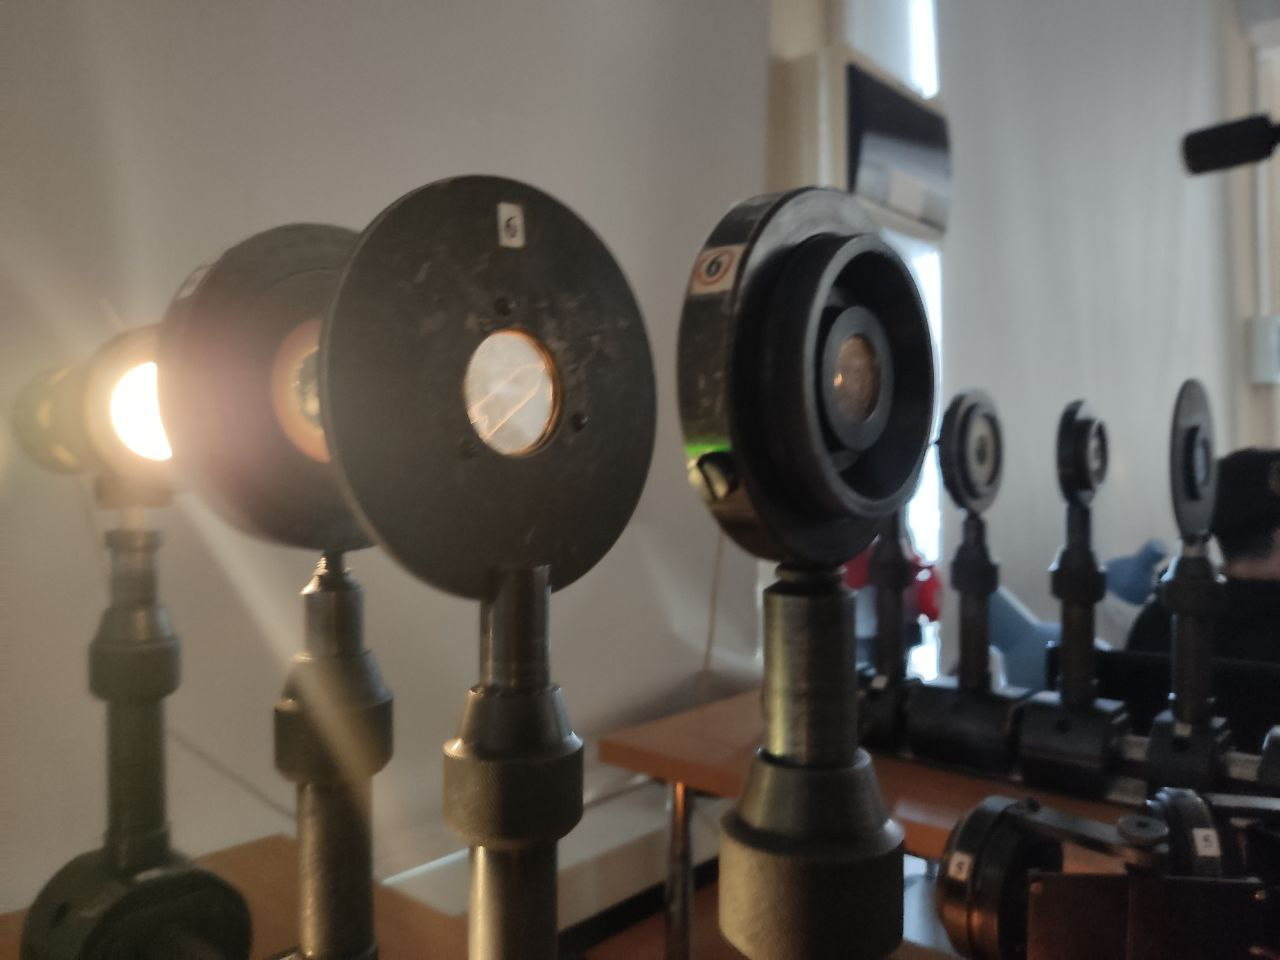
\includegraphics[width=0.35\textwidth]{photo/photo_2024-04-26_17-42-10.jpg}
	\label{fig:boiler}
\end{figure}

\begin{figure}[!h]
	\centering
	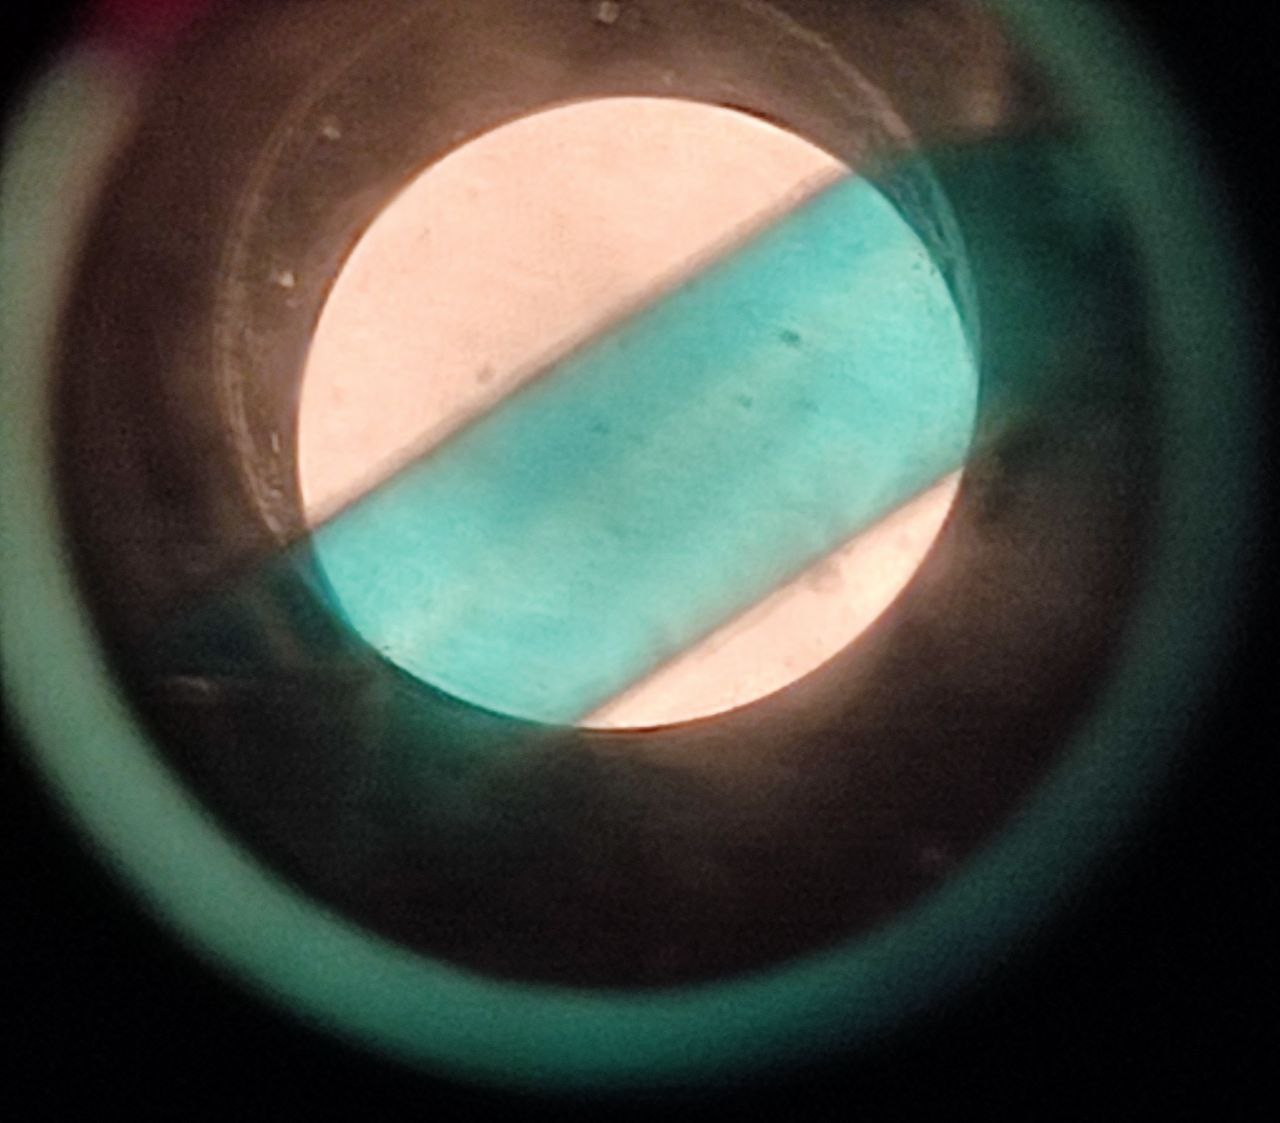
\includegraphics[width=0.35\textwidth]{photo/photo_2024-04-26_17-42-09.jpg}
	\label{fig:boiler}
\end{figure}

\subsection{Интерференция поляризованных лучей}

Расположим между скрещенными поляроидами мозаичную слюдяную пластинку. Она собрана из 4-х узких полосок слюды, лежащих по сторонам квадрата (две полоски «толщиной» $\lambda/4$ и по одной — $\lambda/2$ и $3\lambda/4$).
\par Вращаем пластинку: изменяется интенсивность света с периодичностью $\pi/4$
\par Вращаем второй поляроид: изменяется цвет пластинок также с периодичностью  $\pi/4$.

Расположение пластин в таблице соответствует фото, повернутое на 45 градусов против часовой.

\newpage

\begin{figure}[!h]
	\centering
	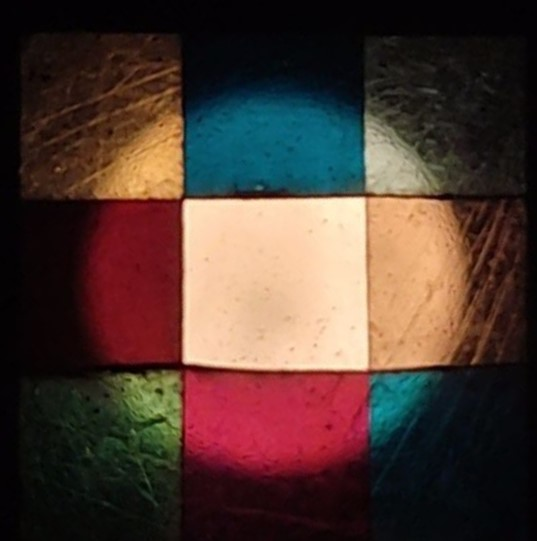
\includegraphics[width=0.6\textwidth]{photo/photo_2024-04-26_17-42-04.jpg}
	\label{fig:boiler}
\end{figure}

.

    \begin{table}[h]
    \centering
    \vspace{0.1cm}
    \label{tab:my_label}
    \begin{tabular}{ |p{2.5cm}|p{2.5cm}|p{2.5cm}|}
 \hline
 $0$ & $\lambda/4$ & $\lambda/4$\\
\hline
 $\lambda/4$ & 0 & $\lambda/2$ \\
\hline
 $\lambda/2$ & $3\lambda/4$ & $\lambda/4$ \\
\hline
 
\end{tabular}
\end{table}

\subsection{Определение направления вращения светового вектора в эллиптически поляризованной волне}

 Снова поставим зелёный фильтр,
а за ним между скрещенными поляроидами
— пластинку произвольной толщины (
$\lambda/4$ ).

Направление вращения - против часовой стрелки.

1) Получим эллиптически-поляризованный свет. Для этого установим разрешённое направление первого поляроида под углом 10–20$^\circ$ к горизонтали так, чтобы вектор \textbf{E} падающего на пластинку света был расположен в первом квадранте.

2) Установим разрешённое направление второго поляроида вертикально и, вращая пластинку, найдем минимальную интенсивность света, прошедшего черех второй поляроид. Вращая второй поляроид, убедимся, что свет поляризован эллиптически, а не линейно. Таким образом, получим эллипс поляризации с вертикально ориентированной малой осью.

3)  Для определения направления вращения светового вектора в эллипсе
установим между поляроидами дополнительную пластинку $\lambda/4$ с известными направлениями «быстрой» и «медленной» осей, ориентированными по осям эллипса поляризации анализируемого света.
В этом случае вектор \textbf{E} на выходе будет таким, как если бы свет прошёл две
пластинки $\lambda/4$: свет на выходе из второй пластинки будет линейно поляризован. Если пластинки поодиночке дают эллипсы, вращающиеся в разные стороны, то поставленные друг за другом, они скомпенсируют
разность фаз, и вектор \textbf{E} на выходе останется в первом
и третьем квадрантах. Если
же световой вектор перешёл в смежные квадранты, значит, эллипсы вращаются в одну сторону. 
\par После второго поляроида интенсивность света максимальна. Значит, две пластины усиливают друг друга, световой вектор перешёл в смежные квадранты, эллипсы вращаются в одну сторону.






%\begin{center}
%\begin{tabular}{|c|c|c|c|}
%\hline 
%\multicolumn{2}{|c|}{$h_\text{ман}$, мм} & $\sigma, \frac{\text{мН}}{\text{К}}$ & T, $^\circ$C \\
%\hline
%188.0 & 188.0 & $(64.5 \pm 3.9)$ & 22\\
%187.0 & 187.0 & $(64.0 \pm 3.9)$ & 30\\
%185.5 & 186.0 & $(63.3 \pm 3.9)$ & 35\\
%184.0 & 184.5 & $(62.5 \pm 3.9)$ & 40\\
%182.5 & 183.0 & $(61.7 \pm 3.9)$ & 45\\
%181.0 & 181.0 & $(60.8 \pm 3.8)$ & 50\\
%179.0 & 179.5 & $(59.9 \pm 3.8)$ & 55\\
%177.5 & 177.5 & $(59.0 \pm 3.8)$ & 60\\
%\hline
%\end{tabular}
%\end{center}
%
%
%Найдем угловые коэффициенты прямых для каждой установки по МНК.
%
%\[
%	a = \frac{<x_i y_i> - < x > < y_i >}{< x_i^2> - < x_i >^2}
%\]
%
%\[
%	b = < \nu_i > - a < N_i >
%\]
%
%Также рассчитаем их погрешности
%
%\begin{equation}
%	S_a^2 = \frac{< x_i^2>}{< x_i^2 > - < x_i >^2} \cdot \frac{<  b_i - b > ^2}{n - 2}
%\end{equation}
%
%
%\begin{center}
%	\Large $q(T)$
%\end{center}

%\begin{figure}[!h]
%	\centering
%	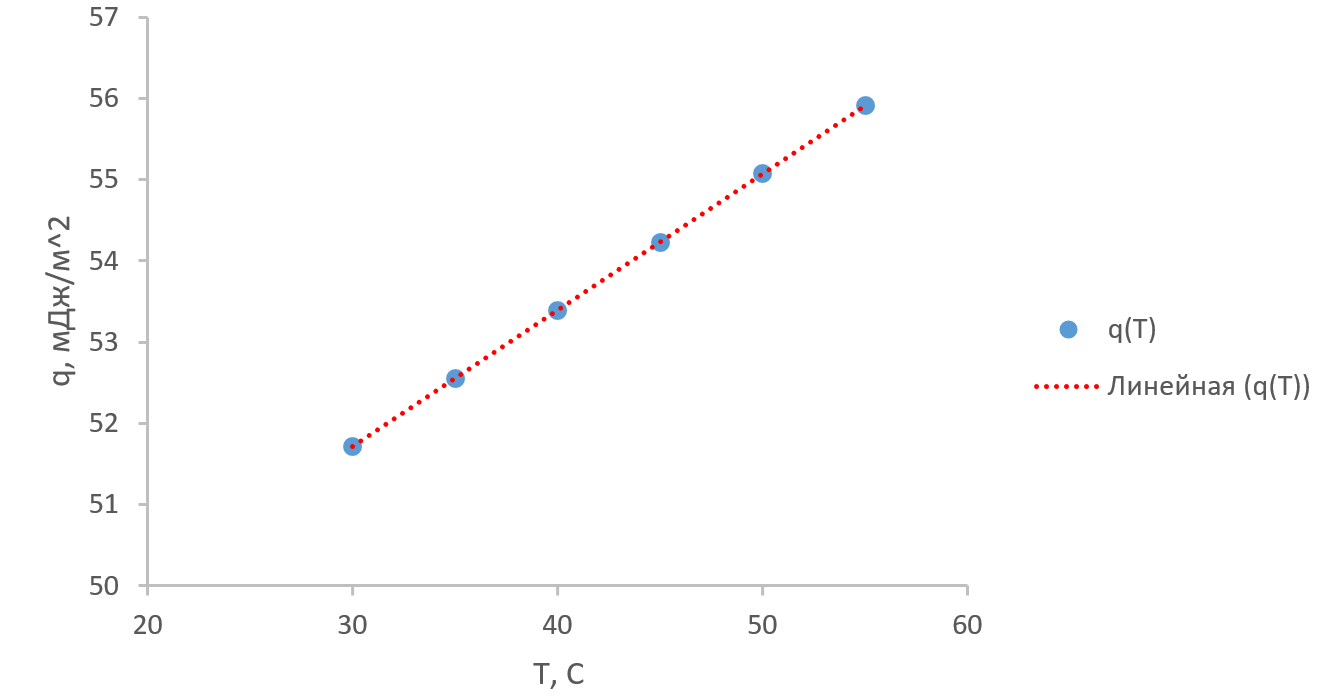
\includegraphics[width=1\textwidth]{2023-02-23_22-23-59.png}
%	\label{fig:boiler}
%\end{figure}

\section{Вывод}

У нас получилось изучить поляризацию и результаты в основном воспроизводимые.

\section{Ресурсы}

Расчет по МНК: метод-наименьших-квадратов.рф


\end{problem}
\end{document}